\section{Kinematics: Describing the Motions of Spacecraft}
\subsection{Introduction to Kinematics}

\subsubsection{Particle Kinematics and Vector Frames}
\label{sub_sec:Particle Kinematics and Vector Frames}
Something with direction and magnitude.

\[
	\begin{aligned}
		\bm{r} & = x \bm{{\hat{e}_{1}}} + y \bm{{\hat{e}_{2}}} + z \bm{{\hat{e}_{3}}} \\
		       & = r \bm{{\hat{e}_{r}}}                                               \\
		       & = \prescript{\mathcal{E}}{}{
			\begin{bmatrix}
				x \\
				y \\
				z
			\end{bmatrix}
		}                                                                             \\
	\end{aligned}
\]

\begin{example}
	Let the frame \(\mathcal{E} \) be defined as: \(\mathcal{E} \colon \{ \hat{e} _1, \hat{e} _2, \hat{e} _3\} \), with the vector, \(\bm{q}  = 3 \bm{{\hat{e}_{1}}} + 2\bm{{\hat{e}_{3}}} \).\\
	Thus, the vector \(\bm{q} \) can be written in matrix form as:
	\[
		\bm{q}  = \prescript{\mathcal{E}}{}{
			\begin{bmatrix}
				3 \\
				0 \\
				2
			\end{bmatrix}
		}
	\]
\end{example}
\subsubsection*{Coordinate Frames}
\label{subsub_sec:Coordinate Frames}
Let a coordinate frame \(\mathcal{B} \) be defined through 3 unit orthogonal vectors, \( \{ \bm{{\hat{b}_{1}}} , \bm{{\hat{b}_{2}}} , \bm{{\hat{b}_{3}}}  \} \). Let the origin of the frame be given by \( \mathcal{O} _\mathcal{B} \). Then the frame is defined as:
\[
	\mathcal{B} \colon \{ \mathcal{O} _\mathcal{B} , \bm{{\hat{b}_{1}}} , \bm{{\hat{b}_{2}}} , \bm{{\hat{b}_{3}}}  \}
\]
Often the frame origin is ignored, and the shorthand notation is used to define the frame as:
\[
	\mathcal{B} \colon \{ \bm{{\hat{b}_{1}}} , \bm{{\hat{b}_{2}}} , \bm{{\hat{b}_{3}}}  \}
\]

\subsubsection*{Angular Velocity}
The angular velocity vector of a rigid body is often defined as:
\[
	\begin{aligned}
		\bm{\omega }                       & = \omega _1 \bm{{\hat{b}_{1}}} + \omega _2 \bm{{\hat{b}_{2}}} + \omega _3 \bm{{\hat{b}_{3}}} \\
		\prescript{\mathcal{B}}{}{\omega } & = \prescript{\mathcal{B}}{}{
			\begin{bmatrix}
				\omega _1 \\
				\omega _2 \\
				\omega _3
			\end{bmatrix}
		}
	\end{aligned}
\]
where, \(\omega _1, \omega _2, \omega _3 \) are the instantaneous angular velocities about the \(\bm{{\hat{b}_{1}}} , \bm{{\hat{b}_{2}}} , \bm{{\hat{b}_{3}}} \) axes respectively. The angular velocity frame components is shown in \autoref{fig:angularVelocityFrameComponents}.
\begin{figure}[H]
	\centering
	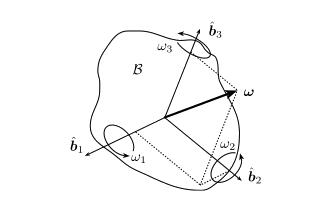
\includegraphics[width=0.5\linewidth]{figures/dynamics/angular_vel.png}
	\caption{Angular velocity body frame components}
	\label{fig:angularVelocityFrameComponents}
\end{figure}

\subsubsection*{Rotation about a Fixed Axis}
Let a body \(\mathcal{B} \) rotate about the axis \(AB\) as shown in \autoref{fig:rotationAboutFixedAxis}. Let the origin \(\mathcal{O} \) of the coordinate system \(\mathcal{B} \) located on the axis of rotation. Let \(P\) be a body fixed point located relative to \(O\) by the vector \(\bm{r} \). Thus, if the vector \(\bm{r} \) is defined in the \(\mathcal{B} \) frame, then the following can be said, from the geometery of the problem:
\[
	\begin{aligned}
		\vert \bm{\dot{r} }  \vert & = (r \sin \theta)  \omega    \\
		\bm{\dot{r} }              & = \bm{\omega } \times \bm{r} \\
	\end{aligned}
\]
\begin{figure}[H]
	\centering
	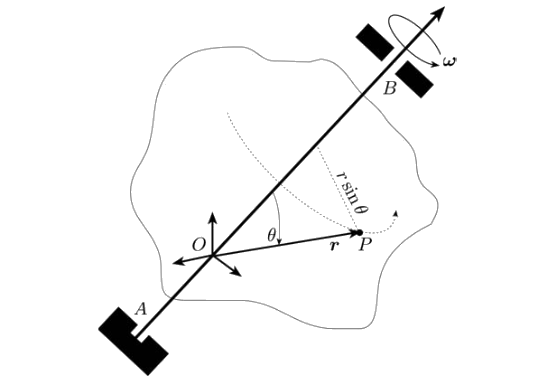
\includegraphics[width=0.5\linewidth]{figures/dynamics/rotationAboutFixedAxis.png}
	\caption{Rotation about a fixed axis}
	\label{fig:rotationAboutFixedAxis}
\end{figure}

\subsubsection{Vector Differentiation and Transport Theorem}
% Vector Differention subsection
\label{subsub_sec:Vector Differentiation}

Let \(\mathcal{N} \) be an inertially fixed frame denoted by the traid, \( \{\bm{{\hat{n}_{1}}}, \bm{{\hat{n}_{2}}}, \bm{{\hat{n}_{3}}}\} \). Let \(\mathcal{B} \) be a another frame denoted by the traid, \( \{\bm{{\hat{b}_{1}}}, \bm{{\hat{b}_{2}}}, \bm{{\hat{b}_{3}}} \}\). For simplicity, the let the origin of the two frames coincide.

Let \(\bm{r}\) be a vector in \(\mathcal{B} \) frame,
\[
	\bm{r} = r_{1}\bm{{\hat{b}_{1}}} + r_{2}\bm{{\hat{b}_{2}}} + r_{3}\bm{{\hat{b}_{3}}}
\]

Let the angular velocity vector \(\omega_{\mathcal{B} / \mathcal{N} }\) define the angular velocity of the \(\mathcal{B} \) frame with respect to the \(\mathcal{N} \) frame. The angular velocity vector is defined usually in the \(\mathcal{B} \) frame as,
\[
	\omega_{\mathcal{B} / \mathcal{N} } = \omega_{1}\bm{{\hat{b}_{1}}} + \omega_{2}\bm{{\hat{b}_{2}}} + \omega_{3}\bm{{\hat{b}_{3}}}
\]
To denote that a derivative of a vector \(\bm{r} \) as seen by the \(\mathcal{B} \) frame, we use the notation,
\[
	\prescript{\mathcal{B}}{}{\frac{d\bm{x}}{{dt}}}{}
\]
The derivative of the vector \(\bm{r} \) as seen by the \(\mathcal{B} \) frame is given by,
\[
	\begin{aligned}
		\prescript{\mathcal{B}}{}{\frac{d\bm{r}}{{dt}}}{dt} & = \prescript{\mathcal{B}}{}{\frac{d}{dt}\left(
			r_{1}\bm{{\hat{b}_{1}}} + r_{2}\bm{{\hat{b}_{2}}} + r_{3}\bm{{\hat{b}_{3}}}
			\right)}                                                                                                                                           \\
		                                                    & =\dot{r}_1 \bm{{\hat{b}_{1}}}  + \dot{r}_2 \bm{{\hat{b}_{2}}} + \dot{r}_3 \bm{{\hat{b}_{3}}}
	\end{aligned}
\]
Since the derivative of the unit vectors \(\bm{{\hat{b}_{i}}}\) wrt the frame \(\mathcal{B} \) is 0.

Using chain rule of differentiation, we can write,
% \[
% 	\prescript{\mathcal{N}}{}{\frac{d}{dt} \bm{r} } =\dot{r}_1 \bm{{\hat{b}_{1}}}  + \dot{r}_2 \bm{{\hat{b}_{2}}} + \dot{r}_3 \bm{{\hat{b}_{3}}} + r_1 \prescript{\mathcal{N}}{}{\frac{d}{dt}\bm{b_1}} + r_2 \prescript{\mathcal{N}}{}{\frac{d}{dt}\bm{b_2} + r_3 \prescript{\mathcal{N}}{}{\frac{d}{dt}\bm{b_3}}}{}{}
% \]
\[
    \leftindex[I]^{\mathcal{N}} {\frac{d}{dt}}
\]
And,
\[
	\prescript{\mathcal{N}}{}{\frac{d}{dt}\bm{{\hat{b}_{i}}} } =  \bm{\omega_{\mathcal{B} / \mathcal{N} }} \times \bm{{\hat{b}_{i}}}
\]
Thus, combining the above two equations, we get,
\[
	\prescript{\mathcal{N}}{}{\frac{d}{dt} \bm{r} } = \prescript{\mathcal{B}}{}{\frac{d\bm{r}}{{dt}}}{} + \bm{\omega_{\mathcal{B} / \mathcal{N} }} \times \bm{r}
\]
\begin{theorem}[Transport Theorem]
	Let \(\mathcal{N} \) and \(\mathcal{B} \) be two frames with a relative angular velocity \(\bm{\omega_{\mathcal{B} / \mathcal{N} }} \). Let \(\bm{r} \) be a generic vector. Then the derivative of the vector \(\bm{r} \) as seen by the \(\mathcal{N} \) frame can be related to the derivative of the vector \(\bm{r} \) as seen by the \(\mathcal{B} \) frame as,
	\[
		\prescript{\mathcal{N}}{}{\frac{d}{dt} \bm{r} } = \prescript{\mathcal{B}}{}{\frac{d\bm{r}}{{dt}}}{} + \bm{\omega_{\mathcal{B} / \mathcal{N} }} \times \bm{r}
	\]
\end{theorem}

\begin{note}
	When writing compact notations, the following will hold,
	\[
		\prescript{\mathcal{N}}{}{\frac{d}{dt}\bm{x} } \equiv \bm{\dot{x} }
	\]
\end{note}

\begin{example}
	\label{ex:planar_transport_thm}
	Find the inertial velocity of the point \(S\) shown in \autoref{fig:planar_transport_thm_ex}
	\begin{figure}[H]
		\centering
		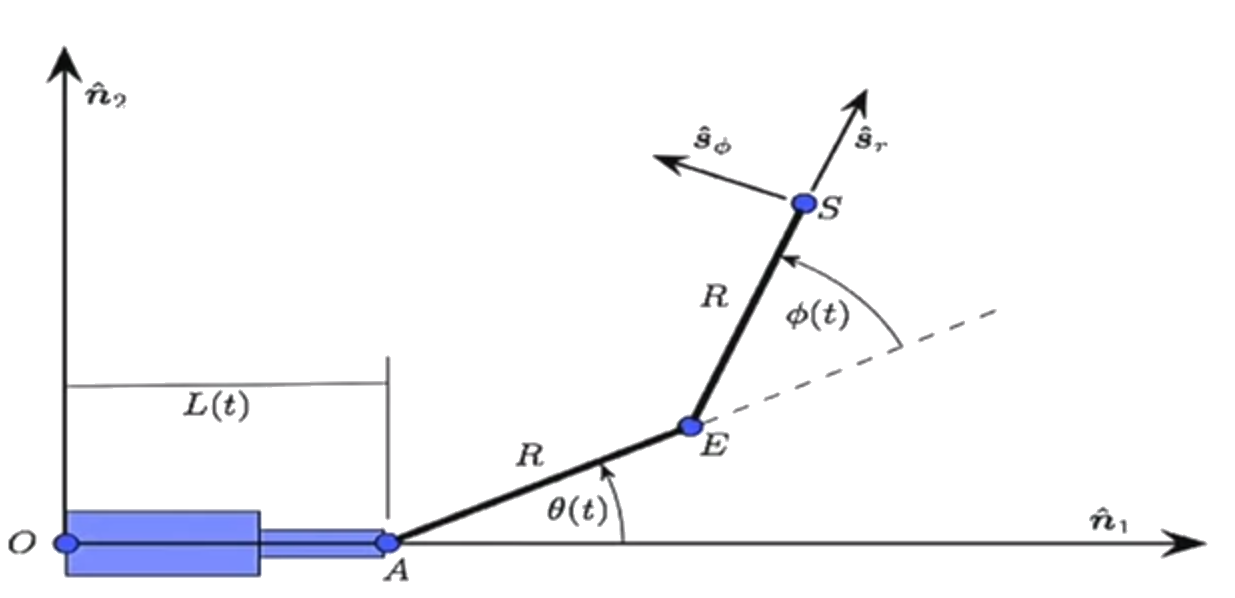
\includegraphics[width=\linewidth]{figures/dynamics/planar_transport_thm_ex.png}
		\caption{Figure for \autoref{ex:planar_transport_thm}}
		\label{fig:planar_transport_thm_ex}
	\end{figure}
	Assigning the frames we have,
	\[
		\begin{aligned}
			\mathcal{N} & \colon  \{ \bm{{\hat{n}_{1}}} , \bm{{\hat{n}_{2}}} , \bm{{\hat{n}_{3}}}  \}       \\
			\mathcal{E} & \colon  \{ \bm{{\hat{e}_{r}}} , \bm{{\hat{e}_{\theta }}} , \bm{{\hat{n}_{3}}}  \} \\
			\mathcal{S} & \colon  \{ \bm{{\hat{s}_{r}}} , \bm{{\hat{s}_{\phi }}} , \bm{{\hat{n}_{3}}}  \}   \\
		\end{aligned}
	\]
	And the angular velocities of the frames relative to each other can be expressed as:
	\[
		\begin{aligned}
			\bm{\omega _{\mathcal{E} / \mathcal{N} }} & = \dot{ \theta} \bm{{\hat{n}_{3}}}                                                    \\
			\bm{\omega _{\mathcal{S} / \mathcal{E} }} & = \dot{ \phi} \bm{{\hat{n}_{3}}}                                                      \\
			\bm{\omega _{\mathcal{S} / \mathcal{N} }} & = \bm{\omega _{\mathcal{E} / \mathcal{N} }}+\bm{\omega _{\mathcal{S} / \mathcal{E} }} \\
			                                          & = (\dot{ \theta} + \dot{ \phi}) \bm{{\hat{n}_{3}}}                                    \\
		\end{aligned}
	\]
	Thus,
	\[
		\begin{aligned}
			\bm{\dot{r} } & = L \bm{{\hat{n}_{1}}} + R \bm{{\hat{e}_{r}}} + R \bm{{\hat{s}_{r}}}                                                                                                                                                                              \\
			              & = \prescript{\mathcal{N}}{}{\frac{d}{dt}\bm{r}} = \prescript{\mathcal{N}}{}{\frac{d}{dt}} L \bm{{\hat{n}_{1}}} + \prescript{\mathcal{E}}{}{\frac{d}{dt}}R \bm{{\hat{e}_{r}}} + \bm{\omega _{\mathcal{E} / \mathcal{N} }} (R \bm{{\hat{e}_{r}}}) +
			\prescript{\mathcal{S}}{}{\frac{d}{dt}}R \bm{{\hat{s}_{r}}} + \bm{\omega _{\mathcal{S} / \mathcal{N} }} (R \bm{{\hat{s}_{r}}})                                                                                                                                    \\
			              & = \dot{L} \bm{{\hat{n}_{1}}} + (\dot{\theta }\bm{{\hat{n}_{3}}} ) \times R \bm{{\hat{e}_{r}}} + \left(
			\dot{\theta}+ \dot{\phi }\right)  \bm{{\hat{n}_{3}}} \times R \bm{{\hat{e}_{r}}}
			\\
			              & = \dot{L}\bm{{\hat{n}_{1}}} + R \dot{\theta } \bm{{\hat{e}_{\theta }}} + R \left(
			\dot{\theta } + \dot{\phi }
			\right)  \bm{{\hat{s}_{\phi }}}
		\end{aligned}
	\]
\end{example}

\begin{example}
	\label{ex:3dtransport_thm}
	Find the inertial velocity of the point \(P\) shown in \autoref{fig:3dtansport_thm_ex}
	\begin{figure}[H]
		\centering
		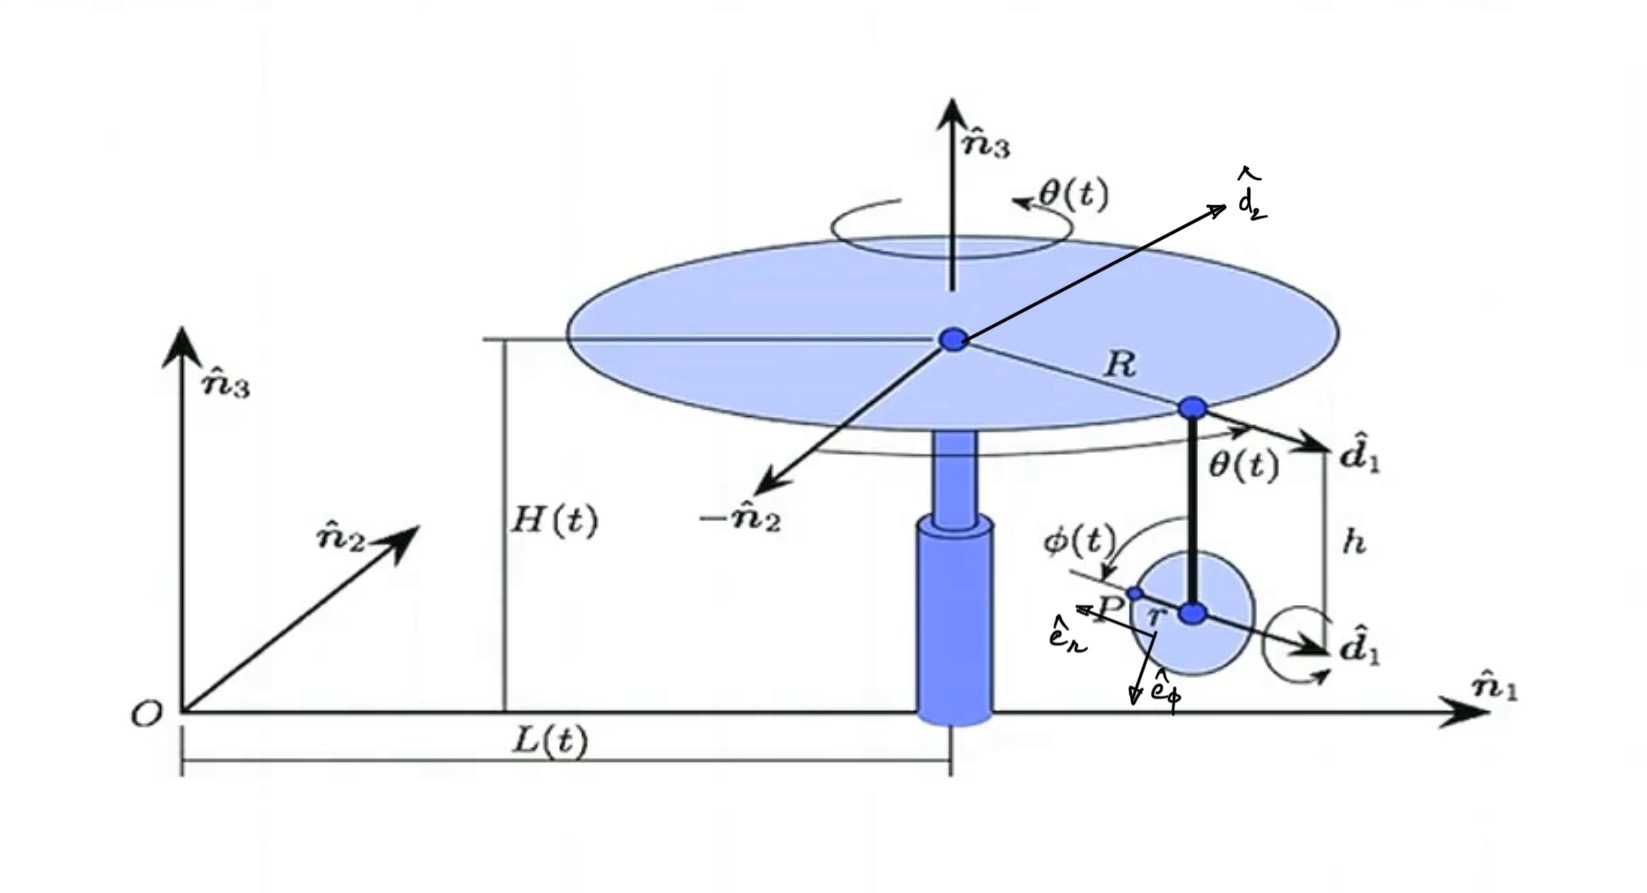
\includegraphics[width=\linewidth]{figures/dynamics/3D_transport_thm_ex.jpg}
		\caption{Figure for \autoref{ex:3dtransport_thm}}
		\label{fig:3dtansport_thm_ex}
	\end{figure}

	Assigning the frames we have,
	\[
		\begin{aligned}
			\mathcal{N} & \colon  \{ \bm{{\hat{n}_{1}}} , \bm{{\hat{n}_{2}}} , \bm{{\hat{n}_{3}}}  \}     \\
			\mathcal{D} & \colon  \{ \bm{{\hat{d}_{1}}} , \bm{{\hat{d}_{2}}} , \bm{{\hat{n}_{3}}}  \}     \\
			\mathcal{E} & \colon  \{ \bm{{\hat{e}_{r}}} , \bm{{\hat{e}_{\phi }}} , \bm{{\hat{d}_{1}}}  \} \\
		\end{aligned}
	\]
	And the angular velocities of the frames relative to each other can be expressed as:
	\[
		\begin{aligned}
			\bm{\omega _{\mathcal{D} / \mathcal{N} }} & = \dot{ \theta} \bm{{\hat{n}_{3}}}                                                    \\
			\bm{\omega _{\mathcal{E} / \mathcal{D} }} & = \dot{ \phi} \bm{{\hat{d}_{1}}}                                                      \\
			\bm{\omega _{\mathcal{E} / \mathcal{N} }} & = \bm{\omega _{\mathcal{D} / \mathcal{N} }}+\bm{\omega _{\mathcal{E} / \mathcal{D} }} \\
			                                          & = \dot{\theta } \bm{{\hat{n}_{3}}} + \dot{\phi } \bm{{\hat{d}_{1}}}                   \\
		\end{aligned}
	\]
	Thus,
	\[
		\begin{aligned}
			\bm{r}  & = L \bm{{\hat{n}_{1}}} + H \bm{{\hat{n}_{3}}} + R \bm{{\hat{d}_{1}}} - h \bm{{\hat{n}_{3}}}  + r \bm{{\hat{e}_{r}}} \\
			\dot{r} & = \prescript{\mathcal{N}}{}{\frac{d}{dt}}\bm{r}                                                                     \\
			        & = \dot{L} \bm{{\hat{n}_{1}}} + \dot{H} \bm{{\hat{n}_{3}}} +
			\left[ \cancelto{0}{
					\prescript{\mathcal{D}}{}{\frac{d}{dt}}R \bm{{\hat{d}_{1}}}
				} + \omega_{\mathcal{D} / \mathcal{N} } \times R \bm{{\hat{d}_{1}}}
				\right]
		\end{aligned}
	\]
\end{example}
